\documentclass{article}
\usepackage[T1]{fontenc}

\usepackage{graphicx}
\usepackage{listings}
\begin{document}

\title{FOSS Lab Report}
\author{Gokul K\\[2\baselineskip]
Roll Number: 21\\[2\baselineskip]}
\date{02 February 2020}

\maketitle

\setcounter{section}{17}
\section{Shell Programming XIV}
\subsection{Aim}
Write a shell script to delete all lines containing a specific word in one or
more file supplied as argument to it.


\subsection{Source Code}
\begin{verbatim}
    #! /bin/bash

    # Gokul K
    # Roll No: 21
    # 25-01-2020

    # Write a shell script to delete all lines containing a specific word in one or
    # more file supplied as argument to it.

    if [[ $# -eq 0 ]]
    then 
        echo "Enter one or more filename(s)"
        exit
    fi

    echo "Enter the word to search"
    read word

    i=1
    for file in "$@"
    do
        cat $file |
        while read line
        do
            if [[ $line != *"$word"* ]]
            then
                echo $line >> .tempfile
            fi
        done
        cat .tempfile > $file
        rm .tempfile
    done

\end{verbatim}

\subsection{Program Description}
The program iterates for each file specified in the argument. Regular
Expression *\$word* is used to match the occurence of word in each line of
the specified files. If found the line is neglected. If not, the line iterates
redirected to a tempfile which will be moved as the original file after completion.

\subsection{Output}
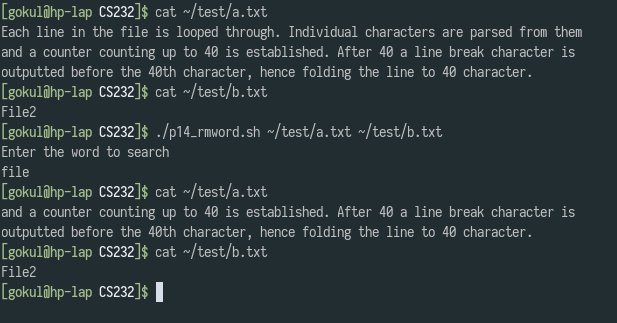
\includegraphics[width=0.9\textwidth]{img/p18.png}\newline

\subsection{Result}
The above program is run on Manjaro Linux shell. Lines found to match with the
pattern where removed from the one or more files specified as input.
\end{document}